% Week 10: the pooled segment cloglog GLMM and its person risk. Input from week10.tex.
\subsection*{From nine segment risks to one person risk}
The who question is about the person: did the participant develop plaque anywhere in the nine trunk
segments (proximal, mid and distal LAD, LCx and RCA)? The segments of one person are not independent,
since risk factors nobody measured act on all of them. The main model is a segment-level cloglog GLMM
with a person random intercept, whose segment risks are pooled into one person risk. A person-level
model of ``any plaque'' is robust but carries little information on effects that act on a few
segments only, such as the LM angle; it is kept as the benchmark. Multiplying the risks of separate
segment models ignores the shared person effect and overestimates the person risk; a logit GLMM gives
no simple person risk; GEE gives none at all; and a count model of segments with plaque cannot use
segment geometry. The pooling rule is fixed before any outcome is seen: the rule alone can move a
person-level AUC by several hundredths, so choosing it afterwards would be a hidden multiple test.

\subsection*{Why the complementary log-log link}
\textbf{One coefficient means the same in every segment.} The pLAD develops plaque far more often than
the dLCx. Under the cloglog link, $e^{\beta}$ is a hazard ratio and multiplies the rate of plaque onset
by the same factor whatever the segment's baseline risk. An odds ratio does not stay fixed: a hazard
ratio of 1.5 is an odds ratio of 1.50 at a baseline risk of 1\,\%, 1.54 at 10\,\% and 1.83 at 50\,\%
(Figure~\ref{fig:hrvsor}).

\textbf{Hazards add, so the nine segments collapse into one number.} Given the person effect, the
probability of no plaque in any segment is $\exp(-\sum_j \Lambda_j)$. The person risk depends on the
tree only through the summed hazard $S_i = \sum_j \Lambda_{ij}$, so the person-level model is itself a
cloglog model, and an unevaluable segment simply drops out of the sum.

\textbf{It matches the data.} Each segment is plaque-free at baseline and seen again about ten years
later, with the onset time unknown. This is grouped survival data, for which the cloglog model is the
proportional hazards model (Prentice and Gloeckler 1978). Log segment length enters as exposure.

The segment model also gives more precise geometry coefficients for local effects, which are seen as
contrasts between segments of the same person; it does not by itself improve discrimination. The cost
is that the person risk is only as good as the segment model: segments independent given the person
effect, a normal person effect and the same hazard ratio in every segment.

\begin{figure}[h]
  \centering
  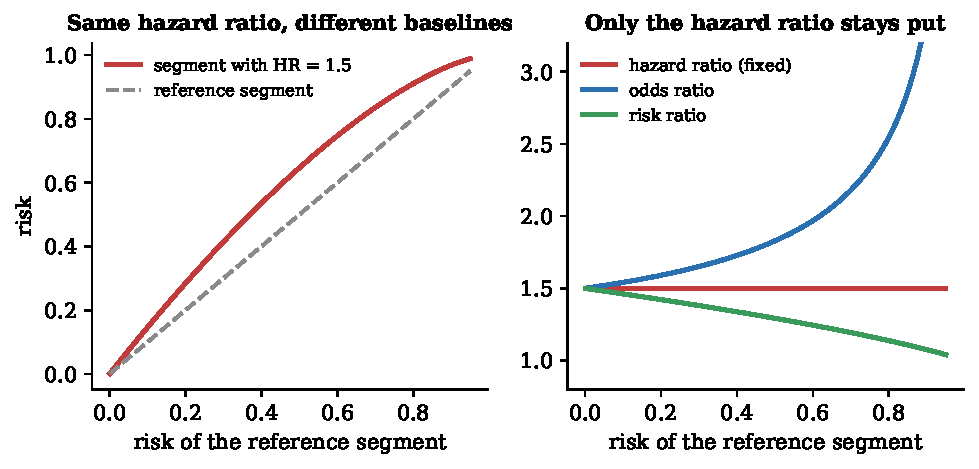
\includegraphics[width=0.85\textwidth]{week_figure/pooled/f06_hr_vs_or.pdf}
  \caption{One risk factor with a fixed hazard ratio of 1.5, made-up numbers. Left: the risk of the
           exposed segment against the risk of the reference segment. Right: the hazard ratio stays
           fixed while the odds ratio and the risk ratio drift with the baseline risk.}
  \label{fig:hrvsor}
\end{figure}

\subsection*{The model}
Each person contributes nine rows, one per trunk segment, with the score
\begin{equation}
  \begin{split}
  \eta_{ij} = {} & \alpha_j + \beta_\mathrm{S}\,\mathrm{SCORE2}_i + \beta_\mathrm{L}\log(\text{length}_{ij})
                 + \beta_\mathrm{c}\, z^\mathrm{curv}_{ij} + \beta_\mathrm{t}\, z^\mathrm{taper}_{ij} \\
               & + \beta_\mathrm{a}\, z^\mathrm{LM\,angle}_i\,[j \in \{\mathrm{pLAD}, \mathrm{pLCx}\}]
                 + \beta_\mathrm{d}\, z^{\mathrm{LM}\to\mathrm{LAD}}_i\,[j \in \mathrm{LAD}]
                 + \beta_\mathrm{x}\, z^{\mathrm{LM}\to\mathrm{LCx}}_i\,[j \in \mathrm{LCx}] .
  \end{split}
  \label{eq:eta}
\end{equation}
$\alpha_j$ is one intercept per segment. Curvature and taper are $z$-scored within segment type. The
three LM features are measured once per person and enter only on the rows downstream of the
bifurcation; $[\cdot]$ is 1 when the condition holds. The five geometry weights form the geometry block.
The segment risk is
\begin{equation}
  P(\text{segment } j \text{ of person } i \text{ develops plaque} \mid b_i)
    = 1 - \exp\!\big(-e^{\eta_{ij} + b_i}\big),
  \qquad b_i \sim N(0, \sigma^2),
  \label{eq:cloglog}
\end{equation}
where the person effect $b_i$ multiplies all nine hazards of a person by $e^{b_i}$. Only $\sigma$ is
estimated. For a new person $b$ is unknown, so the person risk averages over it:
\begin{equation}
  P_i = 1 - \int \exp\!\big(-e^{b} S_i\big)\, \phi(b; 0, \sigma^2)\, \mathrm{d}b ,
  \qquad S_i = \sum_j e^{\eta_{ij}} ,
  \label{eq:personrisk}
\end{equation}
computed by Gauss--Hermite quadrature with 40 points.

\textbf{Worked example (made-up numbers).} Toy person A has a summed hazard $S_\mathrm{A} = 0.763$, of
which the pLAD contributes 0.278. With $\sigma = 1.1$, $P_\mathrm{A} = 0.548$. Setting $b = 0$ gives
0.534, the risk of the median person, and multiplying the average segment risks gives 0.687
(Figure~\ref{fig:shortcuts}). Both shortcuts rank people correctly, so only calibration detects them.
A pLAD hazard ratio of 1.3 raises A's summed hazard by about 11\,\%, not 30\,\%, which is why segment
geometry moves the person risk only a little.

\begin{figure}[h]
  \centering
  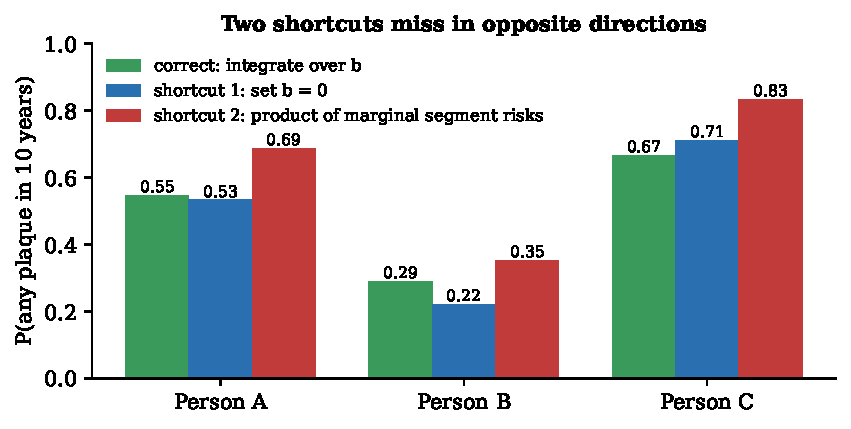
\includegraphics[width=0.75\textwidth]{week_figure/pooled/f16_shortcuts.pdf}
  \caption{Person risk of three made-up people. Green: the correct risk, averaged over the person
           effect $b$. Blue: $b$ set to 0. Red: product of the average segment risks.}
  \label{fig:shortcuts}
\end{figure}

\textbf{Fitting and testing.} The weights and $\sigma$ are fitted by maximum likelihood with $b$
integrated out (L-BFGS-B, Gauss--Hermite quadrature). Cross-validation is split by person, and $P_i$
uses the $\sigma$ from the training folds. Geometry is tested once, by a likelihood-ratio test of the
five geometry weights against the base model (segment intercepts, SCORE2, log length, $\sigma$) on 5
degrees of freedom. The gain in person-level C and the calibration are estimated with intervals, not
tested.

\textbf{Limits.} The current code (\texttt{CGPS\_data/progression\_who\_pooled.py}) runs on the Medis
trees with progression as the outcome and a 2-degree-of-freedom geometry block (mean turning $T_5$ and
the LM angle); taper and the LM diameter ratios wait for the tracer geometry on the plaque-free
cohort. Whether SCORE2 enters as the published score or as refitted factors will be decided in this
model. A gamma person effect, which gives a closed-form risk, is a sensitivity check. The full
derivation is in \texttt{cloglog\_model\_explained.pdf}.
